\documentclass[crop,tikz]{standalone}

\usepackage{pgfplots}
\usepackage{siunitx}
\tikzset{>=latex}

\pgfplotsset{
  inverted/.style = {
    every axis legend/.append style={
      draw=white,
      fill=hardblack,
      text=white
    }
  },
  every non boxed x axis/.append style={
    axis line style={-latex}
  },
  every non boxed y axis/.append style={
    axis line style={-latex}
  }
}

\begin{document}
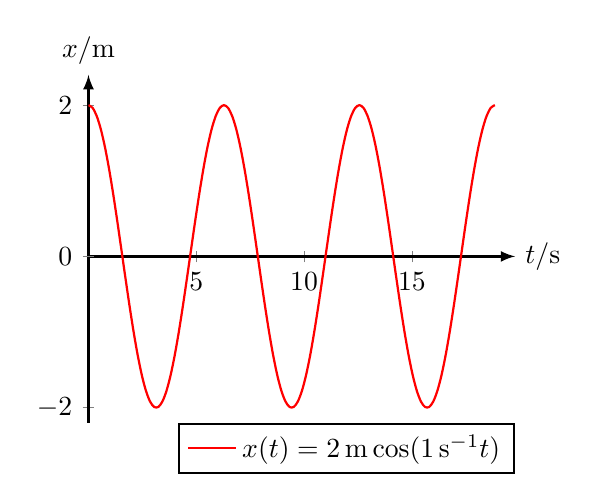
\begin{tikzpicture}
\begin{axis}[
  thick,
  width=7cm,
  height=6cm,
  domain={0}:{6*pi},
  samples=100,
  smooth,
  axis y line=middle,
  axis x line=middle,
  xlabel={$t/\si{\s}$},
  ylabel={$x/\si{\m}$},
  xlabel style={right},
  ylabel style={above},
  xmin=0, xmax={6.3*pi},
  ymin=-2.2, ymax=2.4,
  extra y ticks={0},
  legend cell align={right},
  legend style={at={(1,0)},anchor=north east}
  ]
  \addplot[red] { 2*cos(deg(x)) };
  \addlegendentry{$x(t)=\SI{2}{\m}\cos(\SI{1}{\per\s} t)$};
\end{axis}
\end{tikzpicture}
\end{document}
